\documentclass[11pt, fleqn]{article}

\usepackage{amsmath}
\usepackage{amsfonts}
\usepackage{amsthm}
\usepackage[margin=1in]{geometry} % To set the margin widths
\usepackage{graphicx}
%\usepackage{hyperref}
\usepackage{listings}
\usepackage{multirow}
\usepackage{tabularx}
\usepackage{varioref}
\usepackage{cleveref}  % this redefines vref to use cleverref
\usepackage{siunitx}
%\usepackage{subcaption}
\usepackage{subfig}
\usepackage{titlesec}
\usepackage{bm}

\crefname{equation}{equation}{equations}
\crefname{figure}{figure}{figures}

\sisetup{output-exponent-marker=\textsc{e}}

\titleformat{\section}[block]{\bfseries}{\thesection}{1em}{}


\setlength{\parskip}{12pt} % Sets a blank line in between paragraphs
\setlength\parindent{0pt} % Sets the indent for each paragraph to zero

\begin{document}

\title{Big Data: Homework 4}
\author{Will Clark \& Matthew DeLio \\ 41201-01}
\date{\today}
\maketitle

\section{Node Connectivity Transformation}

Node connectivity (which we are calling \texttt{degree}) is measured by the number of edges for each node in a network. In this context, \texttt{degree} tells us the number of relationships that a household in our population has. We observe in Figure~\ref{fig:degrees} that \texttt{degree} is distributed logarithmically.

\begin{figure}[!htb]
  \centering
  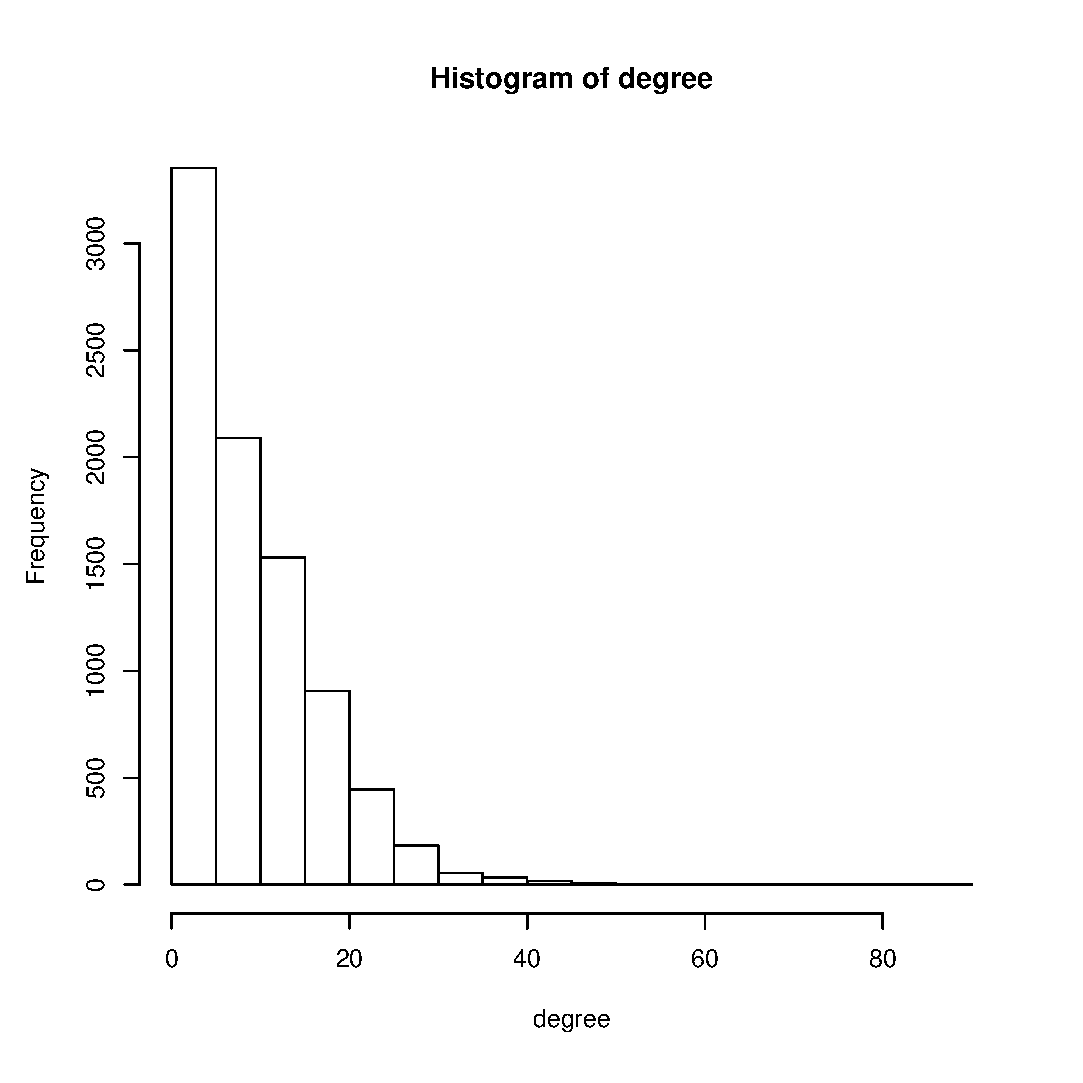
\includegraphics[scale=.5]{degrees.eps}
  \caption{Distribution of \texttt{degree}}
  \label{fig:degrees}
\end{figure}

\section{Predicting Node Connectivity from Controls}
\label{sec:predict}

In this section, we build a model to predict a node's degree by using only our control variables. Our model is: 

\begin{equation} \label{eq:treat}
d(x) = \beta_0 + \bm{X} \bm{\beta} + \nu
\end{equation}

where $d$ is a node's number of degrees, $\bm{X}$ is a vector of control variables including village, religion, type of roof on home, rooms and beds in home, a dummy variable for having electricity in home, whether a home is owned, and whether the person is a ``leader'' in the village. 

We estimate this model using a Gamma-Lasso regression. In Figure~\ref{fig:treat_aic} in the Appendix, we show the Gamma-Lasso path plots with five decision criteria marked: AIC, AICc, BIC, CV.Min, and CV.1se. The $\log(\lambda)$ selected by AICc and by CV.Min are reasonably close to each other (-4.60 and -4.46, respectively, shown in Table~\ref{tab:treat_ic} in the Appendix), which provides us with a confirmation that our model is estimated reasonably well.

We then use the model selected by AICc to predict degree (which we will call $\hat{d}$). We plot $d$ against $\hat{d}$ in Figure~\ref{fig:d_vs_dhat} and see that there is only a very rough correlation between the two ($\sigma_{d,\hat{d}}=0.34$)

\begin{figure}[!htb]
  \centering
  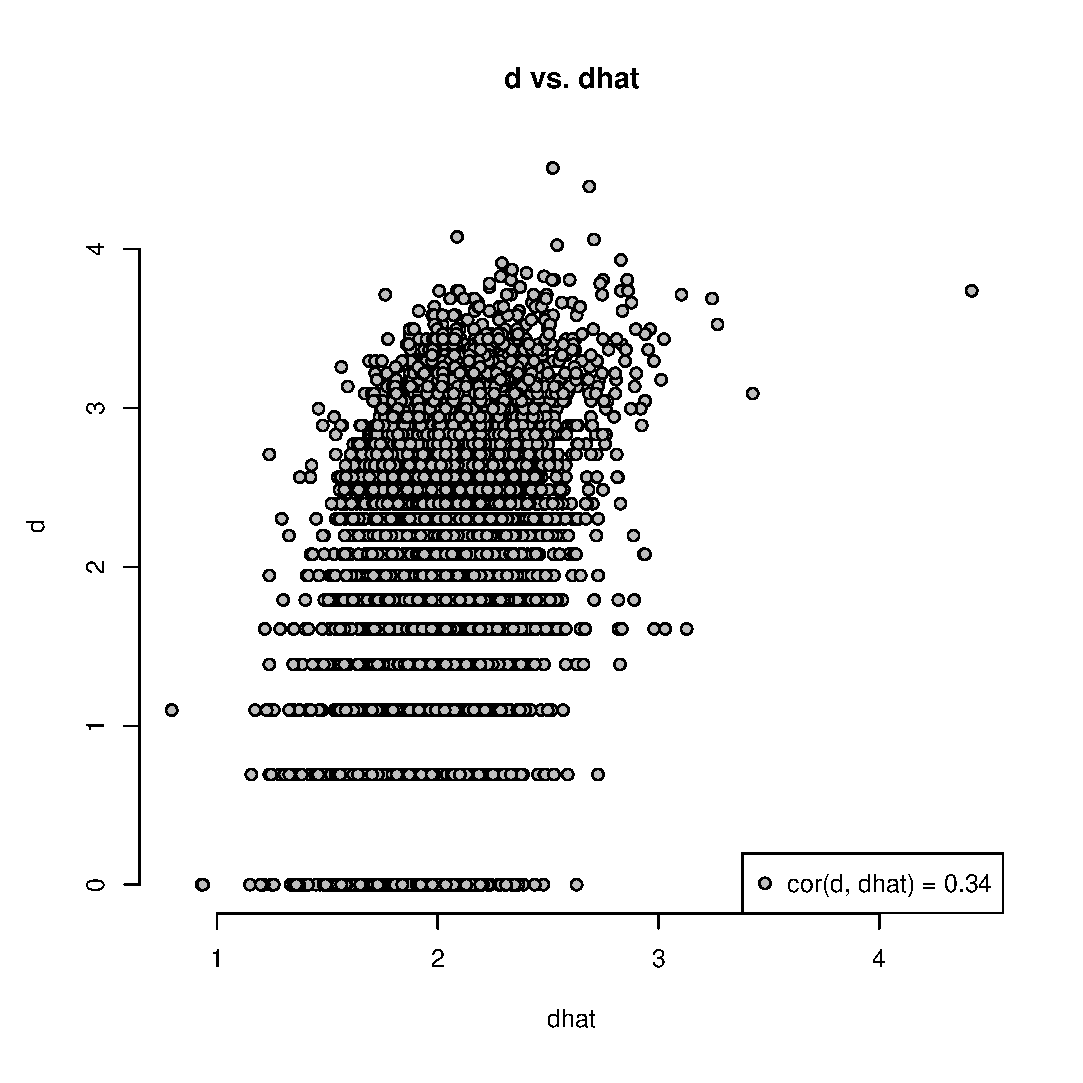
\includegraphics[scale=.5]{d_vs_dhat.eps}
  \caption{Degree and Predicted Degree}
  \label{fig:d_vs_dhat}
\end{figure}

This is a positive result. It tells us that most of the variation in degree, which will be our treatment variable in Section~\ref{sec:model}, is exogenous and cannot be explained by the control variables that we observe. We can therefore measure the effect of degree as a treatment on the propensity to take out a loan and be reasonably sure that we are not simply measuring variation in other observed control variables.

\section{Effect of Node Connectivity on Loan Propensity}
\label{sec:model}

In this section, we use our estimate of predicted degree ($\hat{d}$) to build a model for loan propensity based on node connectivity. We include $\hat{d}$ in our regression model:
\begin{equation} \label{eq:causal}
\log\left(\frac{p}{1-p}\right) = \beta_0 + d \gamma + \hat{d}(x) \delta + \bm{X}\bm{\beta} + \varepsilon
\end{equation}
where $p = \Pr(\text{loan}=1|\bm{X})$. We can substitute in our definition of $\hat{d}(x)$ from equation~\ref{eq:treat}:
\begin{equation}
\log\left(\frac{p}{1-p}\right) = \beta_0 + d \gamma + \left(\beta_0 + \bm{X} \bm{\beta} + \nu\right) \delta + \bm{X}\bm{\beta} + \varepsilon
\end{equation}
which simplifies to
\begin{equation}
\log\left(\frac{p}{1-p}\right) = \beta_0 + \gamma \nu + \hat{d}(x) (\gamma + \delta) + \bm{X}\bm{\beta}
\end{equation}
By estimating the model in equation~\ref{eq:causal}, we can isolate the parameter $\gamma$, which is ultimately the effect of the independent variation in $d$ on the propensity to take out a loan. 

As in Section~\ref{sec:predict}, we use a Gamma-Lasso regression and see that the $\log(\lambda)$ values for the AICc and CV.Min are roughly similar (-5.37 and -5.13, respectively, shown in Table~\ref{tab:causal_ic} and plotted in Figure~\ref{fig:causal_aic} in the Appendix). This tells us our model is reasonably estimated; we proceed using the model chosen by AICc.

The coefficent of interest in this regression is $\gamma$, the effect of exogenous changes in degree connectivity on propensity to take out a loan. In our model, $\gamma$ is 0.0145, which means that having one additional connection (i.e. degree increased by one) increases the odds of taking out a microfinance loan by 1.46 percent\footnote{$100 \cdot \left( \exp(0.0145) - 1 \right) = 1.46$}. This seems like a reasonable estimate \textemdash the coefficient is small but positive, indicating that knowing more people makes one very slightly more likely to take out a loan. We can imagine a story in which information travels more efficeintly to those who are more connected, but it is reasonable to assume that there are much more significant predictors of loan propensity than how many friends a person has.

In Table~\ref{tab:pos} and~\ref{tab:neg}, we see the 5 most positive and negative predictors of loan propensity. 

% latex table generated in R 3.0.2 by xtable 1.7-4 package
% Thu Apr 30 17:16:05 2015
\begin{table}[ht]
\centering
\begin{tabular}{rrr}
  \hline
 & $\beta_j$ & odds multiplier \\ 
  \hline
village4:roofthatch & 0.45 & 56.56 \\ 
  village21:ownershipRENTED & 0.42 & 52.63 \\ 
  village3:ownershipSHARE OWNED & 0.41 & 51.01 \\ 
  village65:ownershipLEASED & 0.41 & 50.95 \\ 
  village1:roofthatch & 0.41 & 50.37 \\ 
   \hline
\end{tabular}
\caption{Most Significant Positive Predictors} 
\label{tab:pos}
\end{table}

% latex table generated in R 3.0.2 by xtable 1.7-4 package
% Thu Apr 30 21:28:00 2015
\begin{table}[ht]
\centering
\begin{tabular}{rllll}
  \hline
 & $x$ & $\beta_j$ & $\Delta$ likelihood & n \\ 
  \hline
1 & village50 & -0.0417 & -4.0834 & 244 \\ 
  2 & village59:roofstone & -0.0441 & -4.3095 & 268 \\ 
  3 & village36 & -0.0442 & -4.3231 & 289 \\ 
  4 & village71:religionhindu & -0.0483 & -4.7140 & 252 \\ 
  5 & village20:roofthatch & -0.0903 & -8.6304 & 5 \\ 
   \hline
\end{tabular}
\caption{Most Significant Negative Predictors} 
\label{tab:neg}
\end{table}


\section{Naive Estimation of Loan Propensity}

\section{Bootstrapping Uncertainty}

\section{Experimental Design}

\section{Appendix}

\begin{figure}[!htb]
  \centering
  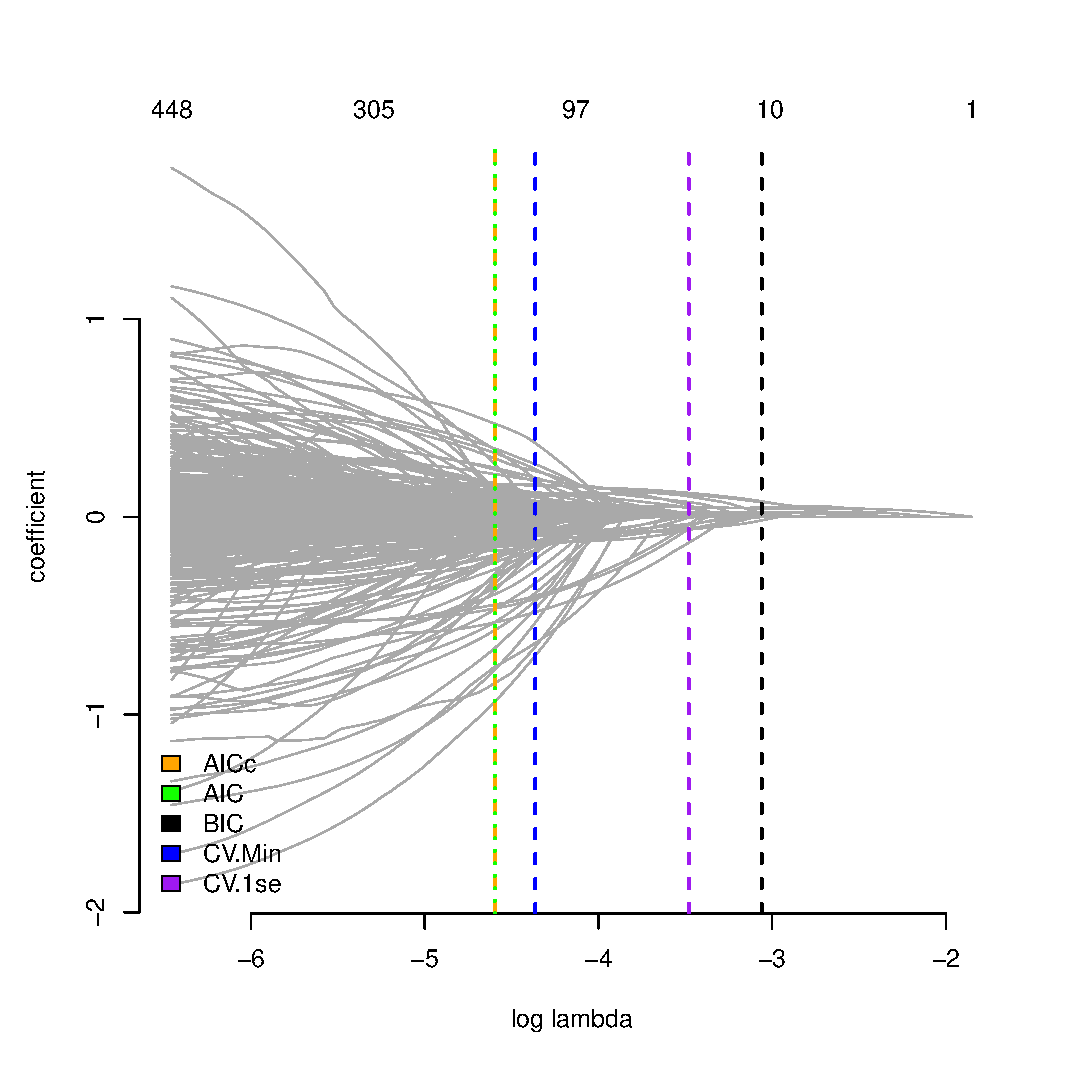
\includegraphics[scale=.5]{treat_aic.eps}
  \caption{Gamma-Lasso Regression for Degree on Controls}
  \label{fig:treat_aic}
\end{figure}

% latex table generated in R 3.0.2 by xtable 1.7-4 package
% Thu Apr 30 15:31:29 2015
\begin{table}[ht]
\centering
\begin{tabular}{rrr}
  \hline
 & $\log(\lambda)$ & Covariates Selected \\ 
  \hline
AICc & -4.60 & 185 \\ 
  AIC & -4.60 & 185 \\ 
  BIC & -3.06 &  10 \\ 
  CV.Min & -4.46 & 161 \\ 
  CV.1se & -3.53 &  37 \\ 
   \hline
\end{tabular}
\caption{Treatment IC Table} 
\label{tab:treat_ic}
\end{table}


\begin{figure}[!htb]
  \centering
  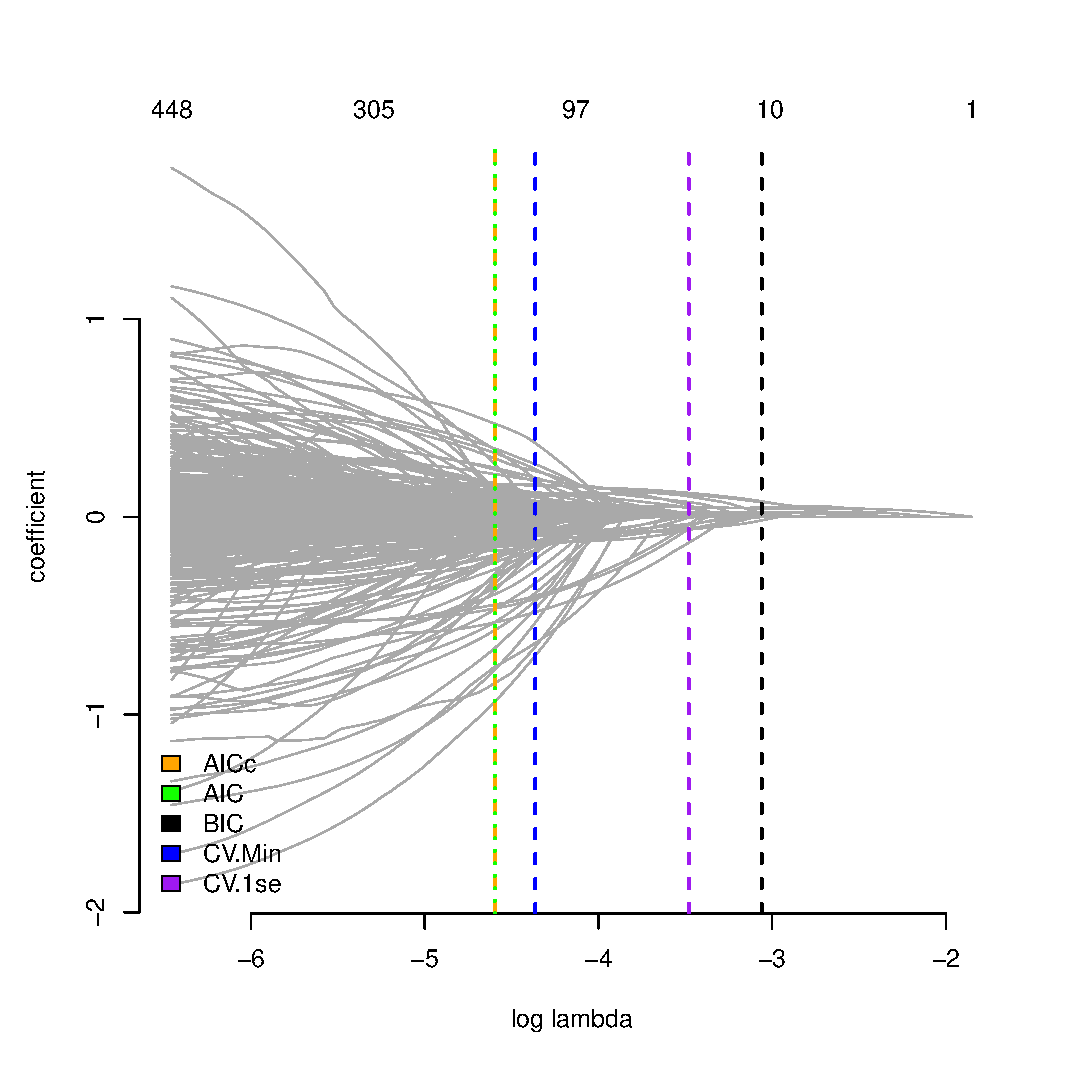
\includegraphics[scale=.5]{treat_aic.eps}
  \caption{Gamma-Lasso Regression for Loan Propensity on Degree}
  \label{fig:causal_aic}
\end{figure}

% latex table generated in R 3.1.2 by xtable 1.7-4 package
% Wed Apr 29 22:13:10 2015
\begin{table}[ht]
\centering
\begin{tabular}{rrr}
  \hline
 & $\log(\lambda)$ & Covariates Selected \\ 
  \hline
AICc & -5.37 & 148 \\ 
  AIC & -5.37 & 148 \\ 
  BIC & -3.97 &  12 \\ 
  CV.Min & -5.13 & 116 \\ 
  CV.1se & -3.60 &   2 \\ 
   \hline
\end{tabular}
\caption{Causal IC Table} 
\label{tab:causal_ic}
\end{table}


\end{document}
